\chapter{Análisis y Especificación del Sistema}
\label{cap:analisis}

Este capítulo especifica el sistema: identifica sus actores, deriva de las Historias de Usuario los requisitos funcionales y no funcionales, detalla los casos de uso y la trazabilidad entre todos ellos, y termina con un modelo conceptual de dominio. Las decisiones de implementación quedan para el capítulo~\ref{cap:diseno-desarrollo}.

\section{Actores del sistema}

El sistema tiene tres actores primarios, las personas que lo usan, y dos secundarios, los servicios externos en los que se apoya la conversación.

El \textbf{Mayor Independiente} ha elegido en el \textit{onboarding} gestionar la aplicación por sí mismo: conversa por voz o por escrito y tiene todos los ajustes en su propio dispositivo. El \textbf{Mayor Vinculado} delega la configuración en un familiar sin perder el acceso a sus ajustes. No dispone del chat hasta que el familiar introduce el código de emparejamiento; a partir de ahí usa la misma pantalla principal y los mismos ajustes que el independiente, salvo los plazos de las conversaciones, que pasan al familiar, y el contacto de emergencia cuando la vinculación lo ha fijado en el propio familiar. Hay dos decisiones que el familiar no puede tomar por él: si se guardan sus conversaciones y qué parte de su análisis comparte. Los dos perfiles de mayor entran con su cuenta de Google o sin registrarse; en el segundo caso, su identidad queda ligada al teléfono hasta que la guarde con su cuenta de Google. El \textbf{Familiar} gestiona la configuración del Mayor Vinculado desde un panel en su propio dispositivo, donde consulta también lo que el mayor haya decidido compartir. Se autentica con correo electrónico y contraseña, porque necesita una cuenta disponible en cualquier terminal.

Los actores secundarios son la \textbf{API de Gemini}, que genera las respuestas conversacionales y analiza cada conversación al cerrarse, y la \textbf{API de Cloud Text-to-Speech}, que sintetiza la voz con la que se pronuncian esas respuestas. UML considera actor a cualquier agente externo que dispara o atiende eventos del sistema, sea o no humano. Los dos se consumen por red, pero solo Gemini condiciona la posibilidad de la conversación (RNF-14): si la síntesis en la nube falla, la respuesta se pronuncia con la voz del propio dispositivo (CU-04).

Los dos perfiles de mayor heredan de un mismo actor, \textit{Mayor}, como recoge la \autoref{fig:actores}. Se diferencian en la \textbf{configuración}, no en la identidad, y esa diferencia es el atributo \code{autonomy} del modelo de datos. Por eso una misma jerarquía de pantallas y un mismo controlador atienden a los dos, y, completado el emparejamiento, solo cambia qué filas de la pantalla de ajustes se muestran.

\begin{figure}[htbp]
    \centering
    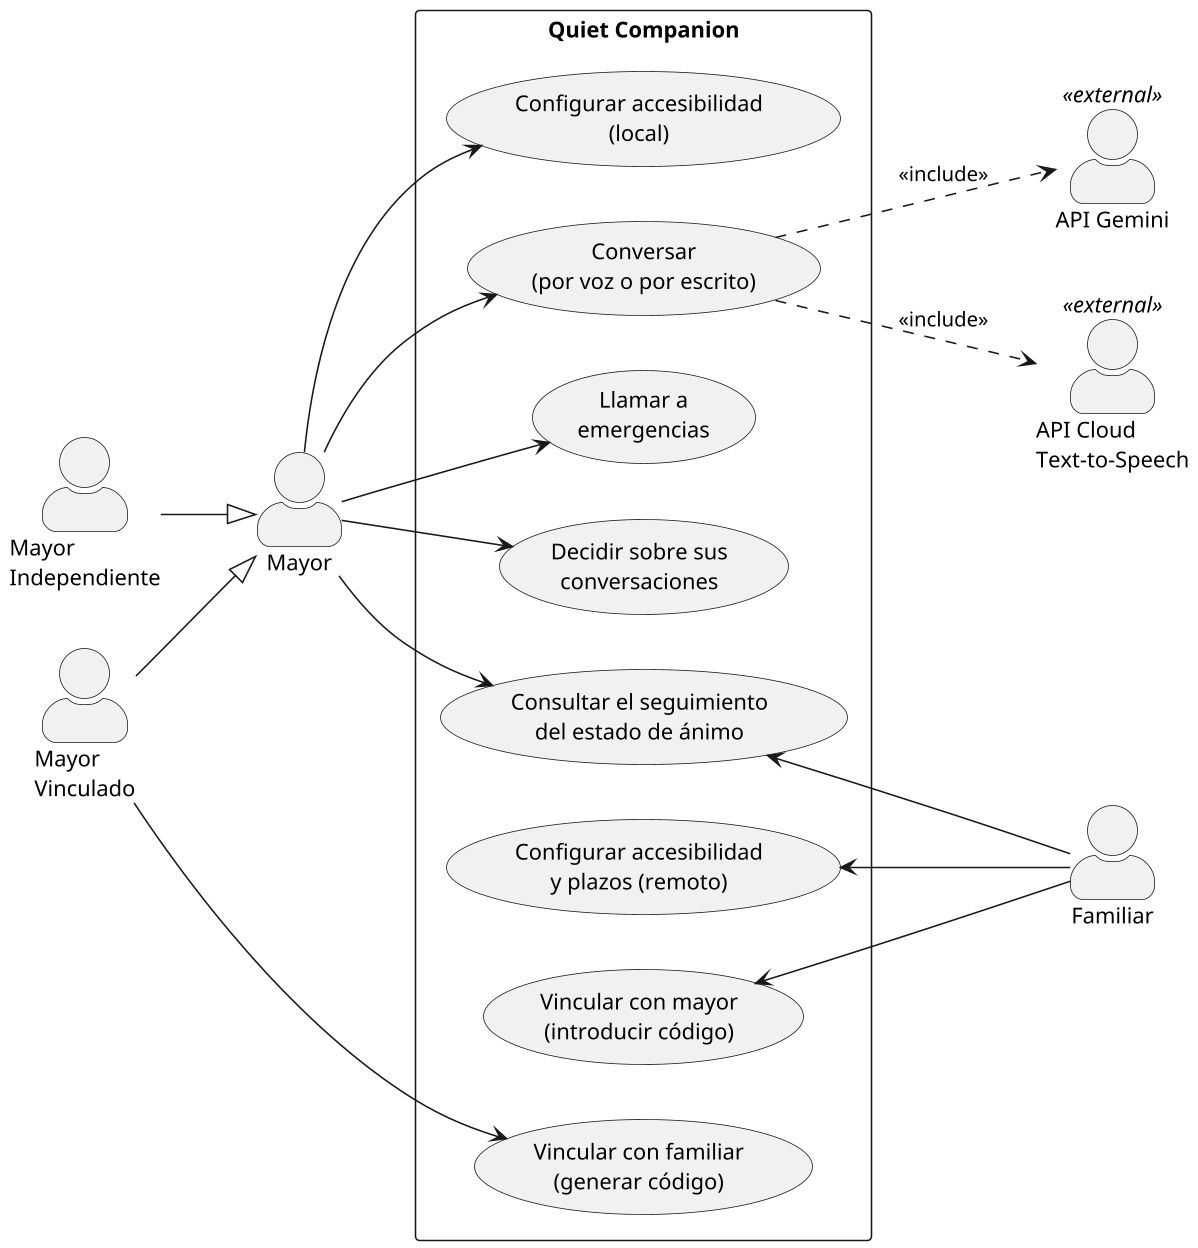
\includegraphics[width=0.8\textwidth]{imagenes/uml/diagrama_actores.png}
    \caption{Diagrama de actores del sistema.}
    \label{fig:actores}
\end{figure}

El diagrama agrupa los casos de uso por objetivo; su especificación, uno a uno, está en el apartado~\ref{sec:casos-de-uso}.

\section{Catálogo de requisitos}
Los requisitos se derivan de las ocho Historias de Usuario y de los tres principios de diseño del capítulo~\ref{cap:introduccion}. Los \textbf{requisitos funcionales} (RF) describen lo que hace el sistema, y los \textbf{no funcionales} (RNF), las condiciones en que debe hacerlo.

\subsection{Historias de Usuario}

La tabla~\ref{tab:enunciado-hu} recoge el enunciado de las ocho Historias de Usuario con el formato habitual de rol, necesidad y beneficio. La tarjeta completa de HU-1, con su estimación y sus criterios de aceptación, aparece como ejemplo en el capítulo~\ref{cap:metodologia}; los criterios de las demás se concretan aquí en requisitos y casos de uso. HU-4 y HU-6 nombran dos roles porque sirven a los dos: la configuración puede ajustarla el mayor o su familiar, y el seguimiento del ánimo lo consultan ambos.


\begin{table}[htbp]
    \centering
    \caption{Enunciado de las Historias de Usuario.}
    \label{tab:enunciado-hu}
    \small
    \begin{tabularx}{\textwidth}{@{}c >{\RaggedRight\arraybackslash}X@{}}
        \toprule
        \textbf{ID} & \textbf{Enunciado} \\
        \midrule
        HU-1 & Como mayor, quiero elegir al abrir la aplicación por primera vez si la gestionaré yo mismo o si me ayudará un familiar, para que el sistema me ofrezca la experiencia adecuada a mis capacidades tecnológicas. \\
        \addlinespace
        HU-2 & Como mayor, quiero conversar con el asistente pulsando un único botón y hablando con naturalidad, para tener compañía sin necesidad de aprender a usar la aplicación. \\
        \addlinespace
        HU-3 & Como mayor con la vista o la destreza mermadas, quiero textos grandes, botones amplios y una única forma de tocar la pantalla, para usar la aplicación sin ayuda. \\
        \addlinespace
        HU-4 & Como familiar, quiero ajustar desde mi móvil la voz del asistente, el volumen, la velocidad de la voz y el tamaño del texto del mayor, y que los cambios le lleguen al momento, para adaptarle la aplicación sin estar a su lado; y como mayor, quiero poder ajustarlos yo mismo. \\
        \addlinespace
        HU-5 & Como mayor, quiero que el asistente recuerde lo que le he contado en conversaciones anteriores, para no tener que repetirlo y sentir que me conoce. \\
        \addlinespace
        HU-6 & Como familiar, quiero saber cómo se ha encontrado el mayor durante la semana, para acompañarle mejor; y como mayor, quiero ver ese mismo resumen, para darme cuenta de cómo me siento y de lo que me preocupa. \\
        \addlinespace
        HU-7 & Como mayor, quiero decidir si se guardan mis conversaciones y qué parte ve mi familiar, y poder cambiarlo cuando quiera, para que nadie sepa de mí más de lo que yo autorice. \\
        \addlinespace
        HU-8 & Como mayor, quiero poder escribir en lugar de hablar cuando no pueda o no quiera usar la voz, para seguir conversando en silencio o cuando el reconocimiento de voz me falle. \\
        \bottomrule
    \end{tabularx}

\end{table}

\subsection{Requisitos funcionales}
Los requisitos funcionales se formalizan según una plantilla común: identificador, nombre, descripción, entradas, salidas, prioridad e Historia de Usuario asociada.

\begin{table}[htbp]
    \centering
    \caption{Requisito Funcional RF-1: Acceso y Selección Inicial de Modo de Uso.}
    \label{tab:rf1}
    \renewcommand{\arraystretch}{1.3}
    \begin{tabular}{|l|>{\raggedright\arraybackslash}p{0.72\textwidth}|}
        \hline
        \multicolumn{2}{|c|}{\textbf{Requisito Funcional: Acceso y Selección Inicial de Modo de Uso}} \\
        \hline
        \textbf{ID} & RF-1 \\
        \hline
        \textbf{Origen} & HU-1 \\
        \hline
        \textbf{Prioridad} & Alta \\
        \hline
        \textbf{Descripción} & Sin sesión iniciada, el sistema debe permitir al mayor entrar con su cuenta de Google o sin registrarse y presentarle después dos opciones excluyentes, usar la aplicación por su cuenta o vincularla con un familiar, y configurar el perfil según la elección. Si la cuenta de Google ya tiene un perfil, debe recuperarlo. \\
        \hline
        \textbf{Entradas} & Forma de acceso y modo elegidos en la pantalla de \textit{onboarding}. \\
        \hline
        \textbf{Salidas} & Perfil de usuario creado en la base de datos con \code{role = elder} y \code{autonomy} $\in$ \{\code{independent}, \code{dependent}\}, o el perfil ya existente de esa cuenta. \\
        \hline
    \end{tabular}

\end{table}

\begin{table}[htbp]
    \centering
    \caption{Requisito Funcional RF-2: Generación y Consumo de Código de Vinculación.}
    \label{tab:rf2}
    \renewcommand{\arraystretch}{1.3}
    \begin{tabular}{|l|>{\raggedright\arraybackslash}p{0.72\textwidth}|}
        \hline
        \multicolumn{2}{|c|}{\textbf{Requisito Funcional: Generación y Consumo de Código de Vinculación}} \\
        \hline
        \textbf{ID} & RF-2 \\
        \hline
        \textbf{Origen} & HU-1 \\
        \hline
        \textbf{Prioridad} & Alta \\
        \hline
        \textbf{Descripción} & Si el mayor opta por el modo vinculado, el sistema debe generar un código corto de 4~caracteres en su dispositivo. El familiar, desde su propio dispositivo, debe poder introducir dicho código para completar el emparejamiento de forma atómica, sin que pueda quedar un estado intermedio en el que solo uno de los dos perfiles esté vinculado. \\
        \hline
        \textbf{Entradas} & Solicitud de generación de código (mayor) e introducción del código (familiar). \\
        \hline
        \textbf{Salidas} & Vinculación bidireccional persistida en la base de datos: el campo \code{linkedCompanionId} en el perfil del mayor y \code{linkedElderId} en el del familiar, ambos escritos dentro de una misma transacción. \\
        \hline
    \end{tabular}

\end{table}

\begin{table}[htbp]
    \centering
    \caption{Requisito Funcional RF-3: Procesamiento Conversacional por Voz.}
    \label{tab:rf3}
    \renewcommand{\arraystretch}{1.3}
    \begin{tabular}{|l|>{\raggedright\arraybackslash}p{0.72\textwidth}|}
        \hline
        \multicolumn{2}{|c|}{\textbf{Requisito Funcional: Procesamiento Conversacional por Voz}} \\
        \hline
        \textbf{ID} & RF-3 \\
        \hline
        \textbf{Origen} & HU-2 \\
        \hline
        \textbf{Prioridad} & Alta \\
        \hline
        \textbf{Descripción} & El sistema debe permitir al mayor mantener una conversación por voz pulsando un único botón central. La entrada de voz se transcribe a texto, se envía al modelo de lenguaje y la respuesta se reproduce mediante síntesis de voz. \\
        \hline
        \textbf{Entradas} & Pulsación del botón principal; señal de audio del usuario. \\
        \hline
        \textbf{Salidas} & Respuesta del asistente reproducida por audio y mostrada en pantalla con tipografía de gran tamaño. \\
        \hline
    \end{tabular}

\end{table}

\begin{table}[htbp]
    \centering
    \caption{Requisito Funcional RF-4: Indicación Visual del Estado del Asistente.}
    \label{tab:rf4}
    \renewcommand{\arraystretch}{1.3}
    \begin{tabular}{|l|>{\raggedright\arraybackslash}p{0.72\textwidth}|}
        \hline
        \multicolumn{2}{|c|}{\textbf{Requisito Funcional: Indicación Visual del Estado del Asistente}} \\
        \hline
        \textbf{ID} & RF-4 \\
        \hline
        \textbf{Origen} & HU-2, HU-3 \\
        \hline
        \textbf{Prioridad} & Alta \\
        \hline
        \textbf{Descripción} & Durante una interacción de voz, el sistema debe comunicar visualmente en qué estado se encuentra, mediante las etiquetas <<Te escucho>>, <<Pensando>> y <<Respondiendo>>. La señalización debe ser perceptible por usuarios con limitaciones visuales moderadas y no puede descansar únicamente en el color. \\
        \hline
        \textbf{Entradas} & Cambios de estado internos del pipeline conversacional. \\
        \hline
        \textbf{Salidas} & Indicador visual y textual en pantalla. \\
        \hline
    \end{tabular}

\end{table}

\begin{table}[htbp]
    \centering
    \caption{Requisito Funcional RF-5: Configuración de Parámetros de Accesibilidad.}
    \label{tab:rf5}
    \renewcommand{\arraystretch}{1.3}
    \begin{tabular}{|l|>{\raggedright\arraybackslash}p{0.72\textwidth}|}
        \hline
        \multicolumn{2}{|c|}{\textbf{Requisito Funcional: Configuración de Parámetros de Accesibilidad}} \\
        \hline
        \textbf{ID} & RF-5 \\
        \hline
        \textbf{Origen} & HU-4 \\
        \hline
        \textbf{Prioridad} & Alta \\
        \hline
        \textbf{Descripción} & El sistema debe permitir configurar la voz del asistente, su volumen y su velocidad, el tamaño del texto y el tiempo de silencio tras el que el asistente da por terminado el turno del mayor. Todo mayor, independiente o vinculado, debe poder ajustarlos desde su propio dispositivo; si está vinculado, su familiar puede cambiar también desde el panel la voz, el volumen, la velocidad y el tamaño del texto. \\
        \hline
        \textbf{Entradas} & Valores de los parámetros configurables. \\
        \hline
        \textbf{Salidas} & Preferencias persistidas en la base de datos y aplicadas en la siguiente interacción del mayor. \\
        \hline
    \end{tabular}

\end{table}

\begin{table}[htbp]
    \centering
    \caption{Requisito Funcional RF-6: Propagación Remota de la Configuración.}
    \label{tab:rf6}
    \renewcommand{\arraystretch}{1.3}
    \begin{tabular}{|l|>{\raggedright\arraybackslash}p{0.72\textwidth}|}
        \hline
        \multicolumn{2}{|c|}{\textbf{Requisito Funcional: Propagación Remota de la Configuración}} \\
        \hline
        \textbf{ID} & RF-6 \\
        \hline
        \textbf{Origen} & HU-4 \\
        \hline
        \textbf{Prioridad} & Alta \\
        \hline
        \textbf{Descripción} & Cuando el familiar modifica las preferencias del mayor desde su panel remoto, los cambios deben propagarse en tiempo real al dispositivo del mayor, sin reiniciar la aplicación y sin que el mayor intervenga. \\
        \hline
        \textbf{Entradas} & Modificación de preferencias en el panel del familiar. \\
        \hline
        \textbf{Salidas} & Actualización efectiva de los parámetros en el dispositivo del mayor. \\
        \hline
    \end{tabular}

\end{table}

\begin{table}[htbp]
    \centering
    \caption{Requisito Funcional RF-7: Memoria Conversacional Contextualizada.}
    \label{tab:rf7}
    \renewcommand{\arraystretch}{1.3}
    \begin{tabular}{|l|>{\raggedright\arraybackslash}p{0.72\textwidth}|}
        \hline
        \multicolumn{2}{|c|}{\textbf{Requisito Funcional: Memoria Conversacional Contextualizada}} \\
        \hline
        \textbf{ID} & RF-7 \\
        \hline
        \textbf{Origen} & HU-5 \\
        \hline
        \textbf{Prioridad} & Media \\
        \hline
        \textbf{Descripción} & Al cerrar cada conversación, el sistema debe extraer de ella los datos estables del mayor (las personas de su entorno y su relación con ellas, dónde vive, sus aficiones o sus rutinas, excepto cualquier dato de salud) junto a un resumen breve, guardarlos en un documento de memoria aparte del registro de conversaciones, e incluir ese documento en el contexto del modelo al empezar la conversación siguiente, para que el asistente tenga en cuenta lo hablado antes. El nombre del mayor, que hace falta en la misma conversación, se aprende en cuanto lo dice. \\
        \hline
        \textbf{Entradas} & Transcripción de la conversación que se cierra y documento de memoria vigente del mayor. \\
        \hline
        \textbf{Salidas} & Documento de memoria actualizado y respuestas del asistente que reflejan el contexto personalizado del usuario. \\
        \hline
    \end{tabular}

\end{table}

\begin{table}[htbp]
    \centering
    \caption{Requisito Funcional RF-8: Catalogación Emocional de las Conversaciones.}
    \label{tab:rf8}
    \renewcommand{\arraystretch}{1.3}
    \begin{tabular}{|l|>{\raggedright\arraybackslash}p{0.72\textwidth}|}
        \hline
        \multicolumn{2}{|c|}{\textbf{Requisito Funcional: Catalogación Emocional de las Conversaciones}} \\
        \hline
        \textbf{ID} & RF-8 \\
        \hline
        \textbf{Origen} & HU-6 \\
        \hline
        \textbf{Prioridad} & Media \\
        \hline
        \textbf{Descripción} & Al terminar una conversación, el sistema debe clasificar el sentimiento general que expresa el mayor (Positivo, Neutro o Negativo), detectar las señales de una lista cerrada que él mismo manifieste (soledad, tristeza, preocupación, malestar físico, desorientación y riesgo), identificar los temas tratados y generar un resumen, todo ello en el servidor y sin almacenar la transcripción. La agregación semanal debe mostrarse al propio mayor (<<Mi semana>>) y, en lo que él autorice, en el panel del familiar. \\
        \hline
        \textbf{Entradas} & Transcripción de la conversación finalizada, retenida únicamente en memoria durante el análisis. \\
        \hline
        \textbf{Salidas} & Sentimiento, señales, temas y resumen almacenados en el registro de la conversación, y agregado semanal visible en la vista del mayor y en el panel de bienestar del familiar. \\
        \hline
    \end{tabular}

\end{table}

\begin{table}[htbp]
    \centering
    \caption{Requisito Funcional RF-9: Consentimiento y Control del Tratamiento Conversacional.}
    \label{tab:rf9}
    \renewcommand{\arraystretch}{1.3}
    \begin{tabular}{|l|>{\raggedright\arraybackslash}p{0.72\textwidth}|}
        \hline
        \multicolumn{2}{|c|}{\textbf{Requisito Funcional: Consentimiento y Control del Tratamiento}} \\
        \hline
        \textbf{ID} & RF-9 \\
        \hline
        \textbf{Origen} & HU-7 (deriva de RNF-10) \\
        \hline
        \textbf{Prioridad} & Alta \\
        \hline
        \textbf{Descripción} & El tratamiento de las conversaciones debe depender de un consentimiento explícito del propio mayor, desactivado por omisión, revocable en cualquier momento con la misma facilidad con que se dio y que el familiar no puede otorgar en su nombre. El mayor debe poder decidir además qué parte del análisis ve su familiar, y esa decisión debe aplicarse en el servidor, no solo en la interfaz. Los plazos de cierre por inactividad y de conservación de los datos derivados deben ser configurables dentro de los márgenes que fije el servidor. \\
        \hline
        \textbf{Entradas} & Gesto explícito del mayor en la pantalla de consentimiento, y ajustes de compartición y de plazos. \\
        \hline
        \textbf{Salidas} & Estado de consentimiento, ámbito de compartición y plazos persistidos en el perfil, y reglas de seguridad que los aplican a toda lectura del familiar. \\
        \hline
    \end{tabular}

\end{table}

\begin{table}[htbp]
    \centering
    \caption{Requisito Funcional RF-10: Conversación por Escrito.}
    \label{tab:rf10}
    \renewcommand{\arraystretch}{1.3}
    \begin{tabular}{|l|>{\raggedright\arraybackslash}p{0.72\textwidth}|}
        \hline
        \multicolumn{2}{|c|}{\textbf{Requisito Funcional: Conversación por Escrito}} \\
        \hline
        \textbf{ID} & RF-10 \\
        \hline
        \textbf{Origen} & HU-8 \\
        \hline
        \textbf{Prioridad} & Baja \\
        \hline
        \textbf{Descripción} & El sistema debe permitir al mayor alternar entre la voz y la escritura con un único botón de la pantalla principal. Un turno escrito debe seguir el mismo camino que uno hablado, también a efectos del análisis al cierre de la conversación, y su respuesta debe mostrarse en pantalla sin leerse en voz alta, salvo que el mayor lo pida. \\
        \hline
        \textbf{Entradas} & Texto introducido en el campo de escritura y pulsación de <<Enviar>>. \\
        \hline
        \textbf{Salidas} & Respuesta del asistente en pantalla con tipografía de gran tamaño, y su locución cuando el mayor pulsa <<Escuchar>>. \\
        \hline
    \end{tabular}

\end{table}

\begin{table}[htbp]
    \centering
    \caption{Requisito Funcional RF-11: Llamada de Emergencia.}
    \label{tab:rf11}
    \renewcommand{\arraystretch}{1.3}
    \begin{tabular}{|l|>{\raggedright\arraybackslash}p{0.72\textwidth}|}
        \hline
        \multicolumn{2}{|c|}{\textbf{Requisito Funcional: Llamada de Emergencia}} \\
        \hline
        \textbf{ID} & RF-11 \\
        \hline
        \textbf{Origen} & Seguridad del mayor (sin Historia de Usuario propia) \\
        \hline
        \textbf{Prioridad} & Media \\
        \hline
        \textbf{Descripción} & El sistema debe permitir al mayor llamar al 112 o a su contacto de emergencia desde la pantalla principal, sin que una pulsación accidental pueda iniciar la llamada. Si el mayor no ha fijado un contacto propio, la vinculación pone como tal a su familiar. \\
        \hline
        \textbf{Entradas} & Pulsación del botón de emergencia y elección del destino. \\
        \hline
        \textbf{Salidas} & Marcador del teléfono abierto con el número escrito. \\
        \hline
    \end{tabular}

\end{table}


\subsection{Requisitos no funcionales (RNF)}

Los requisitos no funcionales se agrupan en seis categorías y se aplican a todo el sistema salvo que se indique lo contrario.


\subsection*{Usabilidad y accesibilidad}
\begin{itemize}
    \item \textbf{RNF-1. Cumplimiento WCAG~2.2.} La interfaz dirigida al mayor debe cumplir los criterios de éxito de nivel~AA de la norma WCAG~2.2 \citep{wcag}, en particular los relativos a perceptibilidad (contraste, tamaño de texto) y operabilidad (área activa de elementos táctiles, ausencia de gestos complejos).
    \item \textbf{RNF-2. Áreas táctiles mínimas.} Todo elemento interactivo de la interfaz del mayor debe tener un área activa de al menos $80 \times 80$ píxeles lógicos.
    \item \textbf{RNF-3. Tipografías mínimas.} El texto de cuerpo en la interfaz del mayor debe presentarse a un tamaño mínimo de 20~sp y los títulos a un mínimo de 28~sp, sujetos al multiplicador definido por el usuario en sus preferencias.
    \item \textbf{RNF-4. Interacciones simples.} La interfaz del mayor debe operarse exclusivamente mediante pulsación simple, excluyéndose el doble toque, la pulsación prolongada y los gestos de deslizamiento.
    \item \textbf{RNF-5. Idioma.} Todos los textos de la interfaz, así como las entradas y salidas de voz, deben presentarse en español de España (es-ES).
\end{itemize}

\subsection*{Rendimiento}
\begin{itemize}
    \item \textbf{RNF-6. Plataforma objetivo.} El sistema debe ejecutarse correctamente en dispositivos Android con \code{minSdk = 24} (Android~7.0), que cubre los terminales de gama media y baja de 2016 en adelante.
    \item \textbf{RNF-7. Latencia de respuesta conversacional.} La latencia percibida entre el fin de la entrada de voz del usuario y el inicio de la respuesta sintetizada no debería superar los 3~segundos en condiciones normales de red y tras superar el \textit{cold start} en caso de haberlo.
\end{itemize}

\subsection*{Seguridad}
\begin{itemize}
    \item \textbf{RNF-8. Protección de credenciales de servicios externos.} Las claves de API de los servicios externos, en particular la de Gemini, no deben residir en el binario que se distribuye al usuario.
    \item \textbf{RNF-9. Aislamiento de identidades.} Las escrituras que afectan a documentos de un usuario distinto del autenticado, en particular el emparejamiento entre el mayor y el familiar, deben ejecutarse en un entorno servidor de confianza y no en el cliente.
\end{itemize}

\subsection*{Privacidad y protección de datos}
\begin{itemize}
    \item \textbf{RNF-10. Tratamiento de datos personales.} El sistema trata datos personales: identificadores de cuenta y, cuando los hay, el correo del familiar o el de la cuenta de Google del mayor, que conserva Firebase Authentication y no la base de datos; el nombre del mayor y los teléfonos de contacto; preferencias, resúmenes de las conversaciones, su categorización emocional y lo que el asistente recuerda del mayor. El tratamiento se ajusta al Reglamento General de Protección de Datos \citep{RGPD2016} y aplica los principios de minimización, limitación de la finalidad y limitación del plazo de conservación. En concreto, requiere el consentimiento explícito del mayor (RF-9); la transcripción no se almacena nunca y solo se procesa, de forma transitoria, para obtener el análisis y la memoria; las conversaciones en las que el mayor interviene menos de tres veces no se analizan, y de ellas solo sale del dispositivo la constancia de que existieron; y los datos derivados se borran al cumplirse un plazo configurable, de noventa días por omisión y nunca superior a ciento ochenta.
\end{itemize}

\subsection*{Mantenibilidad}
\begin{itemize}
    \item \textbf{RNF-11. Arquitectura.} El código fuente debe organizarse según el modelo Clean Architecture combinado con Feature-Sliced Design (CFS), con separación estricta entre las capas de presentación, dominio y datos, y sin acoplamiento horizontal entre \textit{features}.
    \item \textbf{RNF-12. Inyección de dependencias.} Los servicios externos y repositorios deben inyectarse en los controladores mediante los proveedores de Riverpod (apartado~\ref{sec:estado-di}), evitando instanciación directa dentro de la lógica de negocio.
    \item \textbf{RNF-13. Calidad estática.} Todo módulo modificado debe superar el análisis estático (\code{flutter analyze}) sin advertencias antes de su integración en la rama principal.
\end{itemize}

\subsection*{Disponibilidad}
\begin{itemize}
    \item \textbf{RNF-14. Dependencia de conectividad.} El sistema necesita conexión a internet para conversar (API de Gemini) y para sincronizar (Firestore). Si la conexión falla, debe avisar al usuario en lugar de fallar en silencio.
\end{itemize}

\section{Casos de uso}
\label{sec:casos-de-uso}
Esta sección especifica los casos de uso del sistema. Los seis primeros corresponden a HU-1 a HU-4, el núcleo de la aplicación, y los cuatro siguientes a HU-5 a HU-8, que se apoyan en él: CU-07 recoge el consentimiento del mayor, CU-08 y CU-09 lo exigen como precondición, y CU-10 añade a la conversación de CU-04 un segundo canal de entrada. CU-11, la llamada de emergencia, no procede de ninguna historia, sino de la seguridad del mayor (RF-11).

\subsection{Diagramas de casos de uso (UML)}

El diagrama de la \autoref{fig:casos-de-uso} agrupa a los dos perfiles de mayor bajo un actor común, del que ambos heredan, para no repetir las asociaciones que comparten; solo la generación del código de vinculación es exclusiva del mayor vinculado. CU-08 se asocia al mayor de forma implícita, porque no lo inicia un gesto suyo sino el final de la conversación.

\subsection{Especificación detallada}

Cada caso de uso se documenta según la plantilla habitual en ingeniería de requisitos \citep{Sommerville2016}: identificador, nombre, actor primario, precondiciones, flujo principal, flujos alternativos y postcondiciones.

\subsection*{CU-01. Seleccionar modo de uso}

\begin{figure}[p]
    \centering
    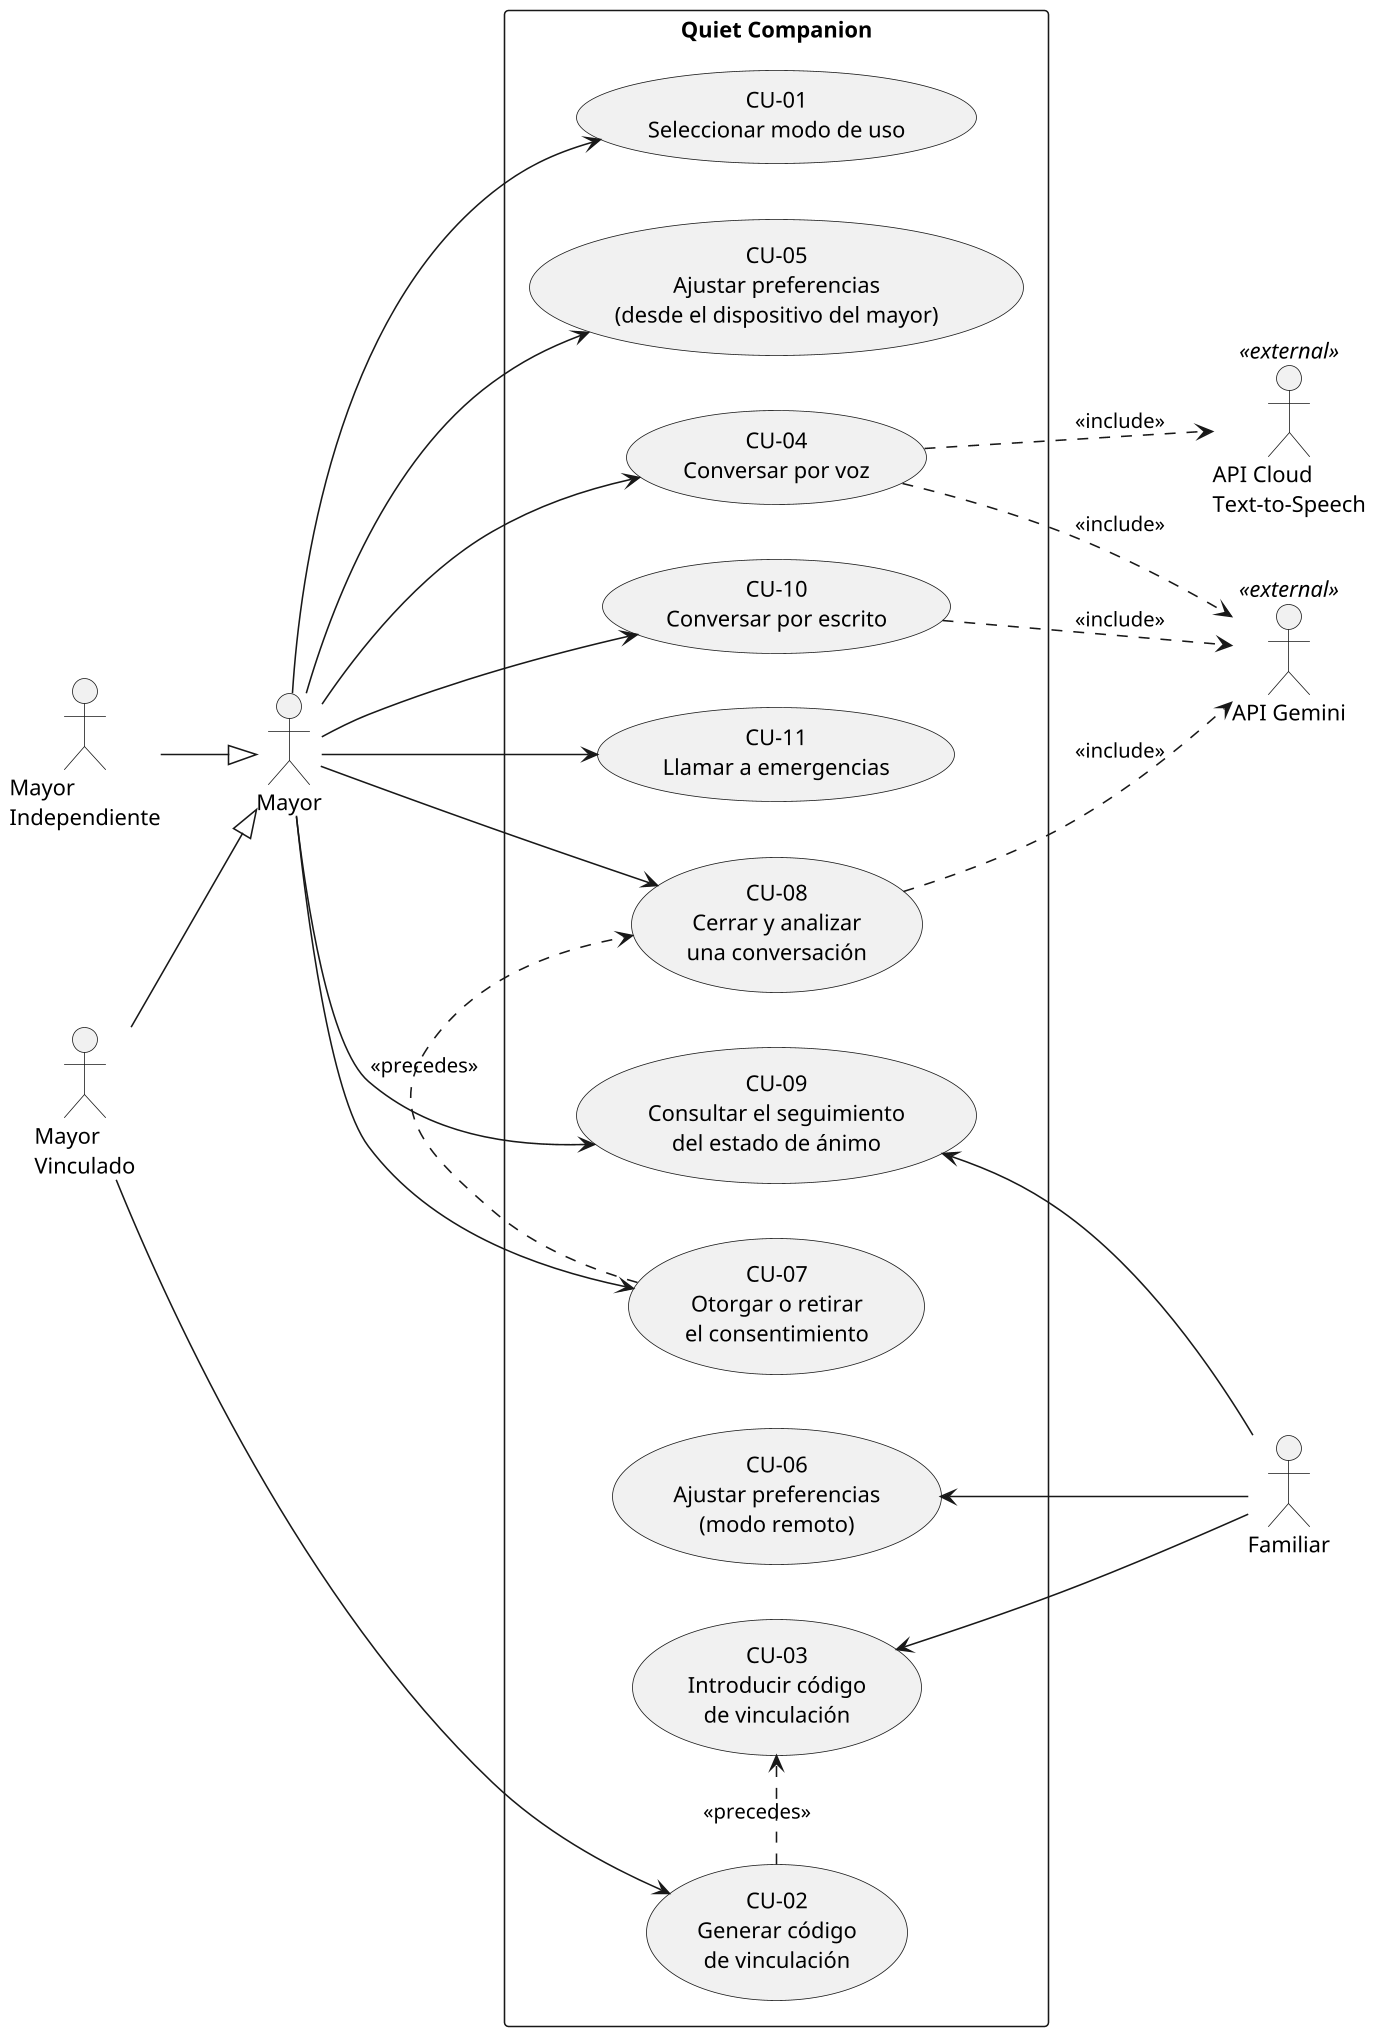
\includegraphics[width=\textwidth, height=0.9\textheight, keepaspectratio]{imagenes/uml/diagrama_casos_de_uso.png}
    \caption{Diagrama de casos de uso del sistema (CU-01 a CU-11).}
    \label{fig:casos-de-uso}
\end{figure}

\noindent\textbf{Actor primario:} Mayor (Independiente o Vinculado, según resultado del caso).

\noindent\textbf{Precondiciones:} No hay sesión iniciada: es el primer arranque de la aplicación en el dispositivo, el primero tras reinstalarla o el siguiente a cerrar la sesión.

\noindent\textbf{Flujo principal:}
\begin{enumerate}[nosep]
    \item El sistema pregunta cómo entrar, con dos botones de gran tamaño: \textit{<<Entrar con Google>>} y \textit{<<Entrar sin registrarme>>}.
    \item El usuario elige una de las dos vías; con Google, elige además su cuenta en el selector del teléfono.
    \item El sistema presenta dos botones de gran tamaño: \textit{<<Usar por mi cuenta>>} y \textit{<<\hspace{0pt}Vincular con mi familiar>>}.
    \item El usuario pulsa una de las dos opciones.
    \item El sistema crea el perfil en la base de datos con \code{role = elder}.
    \item Si la opción seleccionada es la primera, el sistema asigna \code{autonomy = independent} y presenta la pregunta del consentimiento (CU-07) antes de la pantalla principal.
    \item Si la opción seleccionada es la segunda, el sistema asigna \code{autonomy = dependent} y desencadena el caso de uso CU-02.
\end{enumerate}

\noindent\textbf{Flujos alternativos:}
\begin{itemize}[nosep]
    \item \textbf{2a.} La cuenta de Google ya tiene un perfil de mayor, por ejemplo el de un teléfono anterior: el sistema lo recupera tal cual y lleva al mayor a su pantalla principal.
    \item \textbf{2b.} La cuenta de Google es la de un familiar: el sistema cierra la sesión, lo avisa y vuelve al paso~1.
\end{itemize}

\noindent\textbf{Postcondiciones:} Existe un perfil de mayor en la base de datos con su \code{autonomy} definida.

\bigskip

\subsection*{CU-02. Generar código de vinculación}

\noindent\textbf{Actor primario:} Mayor Vinculado.

\noindent\textbf{Precondiciones:} Se ha completado CU-01 con \code{autonomy = dependent}.

\noindent\textbf{Flujo principal:}
\begin{enumerate}[nosep]
    \item El sistema genera un código aleatorio de 4~caracteres (alfanumérico, excluidos los caracteres confundibles O, 0, I y~1).
    \item El sistema persiste el código en el perfil del mayor y lo presenta en pantalla con tipografía de gran tamaño.
    \item El mayor permanece en esa pantalla, sin acceso todavía a la conversación, hasta que el familiar introduce el código (CU-03); entonces la pantalla avanza sola.
\end{enumerate}

\noindent\textbf{Flujos alternativos:}
\begin{itemize}[nosep]
    \item \textbf{3a.} El mayor pulsa <<Cancelar>>: el código se borra de su perfil y vuelve a la elección de modo (CU-01).
\end{itemize}

\noindent\textbf{Postcondiciones:} Existe un código de vinculación activo en el perfil del mayor, pendiente de ser consumido por un familiar.

\bigskip

\subsection*{CU-03. Introducir código de vinculación}

\noindent\textbf{Actor primario:} Familiar.

\noindent\textbf{Precondiciones:} El familiar tiene una cuenta autenticada (correo + contraseña) y posee un código de vinculación válido proporcionado por el mayor.

\noindent\textbf{Flujo principal:}
\begin{enumerate}[nosep]
    \item El familiar accede a la pantalla de emparejamiento desde su dispositivo.
    \item El familiar introduce el código de 4~caracteres.
    \item El sistema valida en el servidor que el código existe y no ha sido consumido, y comprueba que quien solicita la vinculación es un familiar registrado.
    \item El sistema ejecuta una operación atómica que actualiza, en una misma transacción, el campo \code{linkedCompanionId} del mayor y el campo \code{linkedElderId} del familiar, y consume el código para que no pueda reutilizarse.
    \item El sistema confirma la vinculación al familiar, y la aplicación del mayor deja la pantalla del código automáticamente.
\end{enumerate}

\noindent\textbf{Flujos alternativos:}
\begin{itemize}[nosep]
    \item \textbf{3a.} Código inexistente o ya consumido: el sistema muestra mensaje de error y permite     reintentar.
\end{itemize}

\noindent\textbf{Postcondiciones:} Mayor y familiar están vinculados en los dos sentidos y el código ha quedado consumido. El mayor pasa a la pregunta del consentimiento (CU-07) antes de la pantalla principal.

\bigskip

\subsection*{CU-04. Conversar por voz}

\noindent\textbf{Actor primario:} Mayor (cualquier modalidad).

\noindent\textbf{Actor secundario:} API de Gemini y API de Cloud Text-to-Speech.

\noindent\textbf{Precondiciones:} El mayor ha llegado a la pantalla principal (si es vinculado, tras completar CU-03) y el dispositivo tiene conexión a internet.

\noindent\textbf{Flujo principal:}
\begin{enumerate}[nosep]
    \item El mayor pulsa el botón central de micrófono en la pantalla principal.
    \item El sistema solicita permiso de micrófono si no estaba concedido, empieza a escuchar y muestra la etiqueta <<Te escucho>>.
    \item El sistema transcribe lo que dice el mayor con el reconocedor de voz (\code{es-ES}) y da el turno por terminado cuando guarda silencio durante el tiempo elegido en Ajustes.
    \item El sistema muestra <<Pensando>> y envía el texto a la API de Gemini, junto con la instrucción de sistema y lo que el asistente recuerda del mayor (RF-7).
    \item La API de Gemini devuelve una respuesta textual.
    \item El sistema muestra <<Respondiendo>> y la respuesta en pantalla con tipografía de gran tamaño, y se reproduce con la voz, el volumen y la velocidad elegidos. Si la síntesis en la nube falla o tarda, la respuesta se pronuncia con el motor de voz del propio dispositivo.
    \item Al terminar la reproducción, el sistema vuelve al estado de reposo.
\end{enumerate}

\noindent\textbf{Flujos alternativos:}
\begin{itemize}[nosep]
    \item \textbf{1a.} El mayor prefiere escribir: pulsa <<¿Teclado?>> y continúa en CU-10.
    \item \textbf{2a.} El micrófono no está disponible o se deniega el permiso: el sistema muestra <<No se ha podido acceder al micrófono>>, y el mayor puede seguir por escrito (CU-10).
    \item \textbf{4a.} Error de red o de la API: el sistema muestra <<Ups, ha habido un problema de conexión. ¿Puedes repetir?>>, y el micrófono queda listo para volver a intentarlo.
\end{itemize}

\noindent\textbf{Postcondiciones:} La interacción se ha completado o cancelado de forma controlada.

\bigskip

\subsection*{CU-05. Ajustar preferencias (desde el dispositivo del mayor)}

\noindent\textbf{Actor primario:} Mayor (Independiente o Vinculado).

\noindent\textbf{Precondiciones:} El mayor tiene un perfil activo y, si es vinculado, el emparejamiento se ha completado.

\noindent\textbf{Flujo principal:}
\begin{enumerate}[nosep]
    \item El mayor accede a la pantalla de ajustes desde la pantalla principal.
    \item El sistema muestra un menú de cuatro entradas a lo sumo. El mayor elige el tamaño de la letra, o abre el grupo <<Cómo hablamos>>, que reúne la voz, el volumen, la velocidad y el tiempo que el asistente le espera en silencio. Si es independiente, fija además en <<Mis conversaciones>> los plazos de sus conversaciones.
    \item El mayor modifica uno o varios parámetros. Las escalas se presentan como botones grandes (incremento / decremento) con peldaños con nombre, no como deslizadores; la voz, como una lista de cuatro opciones que suenan al tocarlas.
    \item Cada pulsación se persiste por sí sola en la base de datos, sin botón de guardar.
    \item Los nuevos parámetros se aplican inmediatamente a las próximas interacciones de voz y al renderizado de la interfaz.
\end{enumerate}

\noindent\textbf{Flujos alternativos:}
\begin{itemize}[nosep]
    \item \textbf{4a.} El mayor está vinculado y su familiar cambia el mismo parámetro desde el panel (CU-06): prevalece el último cambio, sin arbitraje, porque sobre la accesibilidad ninguno de los dos tiene una autoridad que proteger.
\end{itemize}

\noindent\textbf{Postcondiciones:} Las preferencias del mayor están actualizadas y aplicadas.

\bigskip

\subsection*{CU-06. Ajustar preferencias (modo remoto, desde el Familiar)}

\noindent\textbf{Actor primario:} Familiar.

\noindent\textbf{Precondiciones:} El familiar está vinculado a un mayor, es decir, existen \code{linkedElderId} en su perfil y \code{linkedCompanionId} en el del mayor.

\noindent\textbf{Flujo principal:}
\begin{enumerate}[nosep]
    \item El familiar accede al panel remoto desde su dispositivo.
    \item El sistema muestra el estado actual de las preferencias del mayor (la voz y tres deslizadores, para el volumen, la velocidad y el tamaño del texto) y los plazos de sus conversaciones.
    \item El familiar modifica uno o varios parámetros.
    \item Al soltar cada deslizador, o al elegir una voz o un plazo, el cambio se guarda en la base de datos.
    \item El cambio se propaga en tiempo real al dispositivo del mayor mediante la suscripción reactiva a su documento de usuario, sin que el mayor deba intervenir.
\end{enumerate}

\noindent\textbf{Flujos alternativos:}
\begin{itemize}[nosep]
    \item \textbf{4a.} Error al guardar: el control vuelve a su valor anterior y el panel avisa al familiar.
\end{itemize}

\noindent\textbf{Postcondiciones:} Las preferencias del mayor están actualizadas y aplicadas en su dispositivo.

\bigskip

\subsection*{CU-07. Otorgar o retirar el consentimiento sobre las conversaciones}

\noindent\textbf{Actor primario:} Mayor (Independiente o Vinculado).

\noindent\textbf{Precondiciones:} El mayor ha elegido el modo independiente (CU-01) o ha completado la vinculación (CU-03), y no ha respondido nunca a la pregunta. El consentimiento está desactivado por omisión.

\noindent\textbf{Flujo principal:}
\begin{enumerate}[nosep]
    \item Antes de llegar por primera vez a la pantalla principal, el sistema presenta una pantalla que explica en lenguaje llano qué se guarda, qué no y quién puede verlo: si está vinculado, su familiar, que verá cómo se encuentra y un resumen de lo que hablan; si no, solo él.
    \item El mayor responde <<Sí, quiero>> o <<Ahora no>>, con dos botones del mismo tamaño.
    \item La respuesta se registra mediante una función en la nube, único punto autorizado para escribir ese campo del perfil, junto con la hora del servidor y la versión del texto que el mayor ha leído.
\end{enumerate}

\noindent\textbf{Flujos alternativos:}
\begin{itemize}[nosep]
    \item \textbf{2a.} El mayor responde <<Ahora no>>: la aplicación conversa con normalidad, pero no se analiza ni se guarda nada de lo hablado, y no vuelve a preguntar.
    \item \textbf{3a.} El familiar intenta otorgar el consentimiento en nombre del mayor: el servidor rechaza la operación.
    \item \textbf{*a.} En cualquier momento, desde Ajustes, el mayor puede dar el consentimiento que negó, cambiar qué parte de su análisis ve su familiar o retirarlo. Si lo retira, el análisis se detiene, el familiar pierde al instante el acceso a lo guardado y eso se borra al cumplirse la mitad del plazo de conservación, salvo que el mayor vuelva a consentir antes.
\end{itemize}

\noindent\textbf{Postcondiciones:} El estado del consentimiento y el nivel de compartición quedan guardados y rigen toda lectura posterior.

\bigskip

\subsection*{CU-08. Cerrar y analizar una conversación}

\noindent\textbf{Actor primario:} Mayor, de forma implícita: lo dispara el final de la conversación, no un gesto suyo.

\noindent\textbf{Precondiciones:} Existe una conversación en curso y el mayor ha otorgado el consentimiento (CU-07).

\noindent\textbf{Flujo principal:}
\begin{enumerate}[nosep]
    \item El sistema detecta el final de la conversación: han pasado cinco minutos sin turnos (valor por omisión) o la aplicación ha pasado a segundo plano.
    \item Envía a una función en la nube la transcripción acumulada, que hasta ese momento solo ha existido en la memoria del teléfono.
    \item La función comprueba que el consentimiento sigue vigente y, con una sola llamada al modelo, obtiene el sentimiento, las señales, los temas, un resumen breve y los cambios en la memoria del mayor (RF-7).
    \item Guarda el registro de la conversación (actividad, ánimo y señales) y, en un documento aparte, su contenido (temas y resumen), y actualiza la memoria (\autoref{lst:modelo-datos}).
    \item Descarta la transcripción.
\end{enumerate}

\noindent\textbf{Flujos alternativos:}
\begin{itemize}[nosep]
    \item \textbf{1a.} El mayor sale al marcador de emergencia: la conversación no se cierra y continúa a su vuelta.
    \item \textbf{2a.} El mayor ha intervenido menos de tres veces: solo se envía la constancia de la conversación (inicio, fin y número de turnos), sin texto.
    \item \textbf{3a.} El modelo falla o no responde: la conversación se registra igualmente, con estado de fallo, y la memoria del mayor no se altera.
\end{itemize}

\noindent\textbf{Postcondiciones:} El registro de la conversación y la memoria del mayor quedan actualizados; la transcripción no se ha guardado en ningún soporte.

\bigskip

\subsection*{CU-09. Consultar el seguimiento del estado de ánimo}

\noindent\textbf{Actor primario:} Mayor, en su propia vista de resumen semanal (<<Mi semana>>), o Familiar, en el panel de bienestar.

\noindent\textbf{Precondiciones:} El mayor ha otorgado el consentimiento (CU-07) y existe al menos una conversación analizada. Para el familiar se exige además la vinculación activa.

\noindent\textbf{Flujo principal:}
\begin{enumerate}[nosep]
    \item El actor abre la vista que le corresponde según su rol.
    \item El sistema agrega los registros de conversación de los últimos siete días.
    \item Presenta los días en que hubo conversación, el ánimo predominante y los temas más repetidos; en el panel del familiar, además, las señales detectadas, los resúmenes y lo que el asistente recuerda, según lo que el mayor comparta.
    \item En la vista del mayor, la presentación sigue las restricciones de accesibilidad de HU-3: frases en lugar de gráficas, que además puede escuchar, y la indicación de qué parte de su análisis ve su familiar.
\end{enumerate}

\noindent\textbf{Flujos alternativos:}
\begin{itemize}[nosep]
    \item \textbf{2a.} No hay conversaciones analizadas en los últimos siete días: el sistema lo explica en lugar de mostrar una vista vacía que pudiera tomarse por un error.
    \item \textbf{3a.} El mayor ha restringido lo que comparte: el panel muestra solo lo autorizado y explica por qué falta el resto. La restricción la aplican las reglas de seguridad del servidor, no el cliente.
\end{itemize}

\noindent\textbf{Postcondiciones:} Ninguna. El caso es de solo lectura.

\bigskip

\subsection*{CU-10. Conversar por escrito}

\noindent\textbf{Actor primario:} Mayor (cualquier modalidad).

\noindent\textbf{Actor secundario:} API de Gemini.

\noindent\textbf{Precondiciones:} El mayor tiene un perfil activo y el dispositivo dispone de conexión a internet.

\noindent\textbf{Flujo principal:}
\begin{enumerate}[nosep]
    \item El mayor pulsa <<¿Teclado?>> en la pantalla principal.
    \item El sistema sustituye el botón del micrófono por un campo de texto y un botón <<Enviar>>, y abre el teclado del dispositivo sin necesidad de otro toque.
    \item El mayor escribe su mensaje y pulsa <<Enviar>>.
    \item El sistema cierra el teclado, muestra el estado <<Pensando>> y envía el texto al modelo de lenguaje como un turno más de la conversación en curso.
    \item El sistema muestra la respuesta en pantalla con tipografía de gran tamaño, sin leerla en voz alta.
    \item Si el mayor pulsa <<Escuchar>>, el sistema lee la respuesta, y el botón pasa a <<Parar>> mientras suena.
\end{enumerate}

\noindent\textbf{Flujos alternativos:}
\begin{itemize}[nosep]
    \item \textbf{1a.} El micrófono estaba escuchando: lo oído se descarta sin enviarse.
    \item \textbf{4a.} Error de red o de la API: el sistema muestra un mensaje accesible y devuelve el texto al campo, para no obligar a escribirlo de nuevo.
    \item \textbf{6a.} El mayor pulsa <<¿Hablar?>>: el sistema vuelve al modo de voz (CU-04).
\end{itemize}

\noindent\textbf{Postcondiciones:} El turno escrito forma parte de la conversación en curso y cuenta para su análisis al cierre (CU-08) exactamente igual que uno hablado.

\bigskip

\subsection*{CU-11. Llamar a emergencias}

\noindent\textbf{Actor primario:} Mayor (cualquier modalidad).

\noindent\textbf{Precondiciones:} El mayor ha llegado a la pantalla principal.

\noindent\textbf{Flujo principal:}
\begin{enumerate}[nosep]
    \item El mayor pulsa el botón rojo de emergencia de la pantalla principal.
    \item El sistema abre a pantalla completa la pantalla de emergencia, con <<Llamar al 112>> y, si hay contacto de emergencia, <<Llamar a>> seguido de su nombre.
    \item El mayor elige uno de los dos.
    \item El sistema abre el marcador del teléfono con el número escrito, y el mayor pulsa llamar.
\end{enumerate}

\noindent\textbf{Flujos alternativos:}
\begin{itemize}[nosep]
    \item \textbf{3a.} El mayor pulsa <<Cancelar>>: vuelve a la pantalla principal sin llamar.
    \item \textbf{4a.} El marcador no se puede abrir: el sistema lo avisa en la propia pantalla.
\end{itemize}

\noindent\textbf{Postcondiciones:} Si había una conversación en curso, sigue abierta al volver (CU-08).


\subsection{Trazabilidad}

La tabla~\ref{tab:trazabilidad} cruza Historias de Usuario, requisitos funcionales y casos de uso. Con ella se comprueba que cada requisito y cada caso de uso responde a una necesidad del usuario, y que cada historia, salvo HU-3, tiene al menos un caso de uso que la realiza.

\begin{table}[htbp]
    \centering
    \caption{Trazabilidad entre Historias de Usuario, Requisitos funcionales y Casos de uso.}
    \label{tab:trazabilidad}
    \begin{tabularx}{\textwidth}{@{}c >{\RaggedRight\arraybackslash}X >{\RaggedRight\arraybackslash}X@{}}
        \toprule
        \textbf{Historia de Usuario} & \textbf{Requisitos funcionales} & \textbf{Casos de uso} \\
        \midrule
        HU-1 & RF-1, RF-2                & CU-01, CU-02, CU-03 \\
        HU-2 & RF-3                      & CU-04 \\
        HU-3 & RF-4                      & No procede \\
        HU-4 & RF-5, RF-6                & CU-05, CU-06 \\
        HU-5 & RF-7                      & CU-08 \\
        HU-6 & RF-8                      & CU-08, CU-09 \\
        HU-7 & RF-9                      & CU-07 \\
        HU-8 & RF-10                     & CU-10 \\
        No procede & RF-11               & CU-11 \\
        \bottomrule
    \end{tabularx}

\end{table}

HU-3 no tiene casos de uso propios: sus criterios son restricciones de accesibilidad que afectan a todos los casos de uso del mayor y se recogen como RNF-1 a RNF-4. Su único requisito funcional, RF-4, se cumple dentro de CU-04 y CU-10.

RF-11 y CU-11, la llamada de emergencia, no tienen historia propia: responden a la seguridad del mayor, que ninguna historia formula y que la aplicación no puede dejar sin cubrir.

RF-9 y CU-07 se asignan a HU-7, y no a HU-5 o HU-6, porque el consentimiento responde a una necesidad propia del mayor: decidir qué se guarda de él y quién lo ve. HU-5 y HU-6 dependen de él a través de las precondiciones de CU-08 y CU-09, y RNF-10 recoge las garantías que lo rodean.

\section{Modelo conceptual de dominio}

El modelo conceptual de la \autoref{fig:dominio} recoge las entidades que maneja el sistema y sus relaciones, sin entrar en cómo se implementan.

\begin{figure}[tbp]
    \centering
    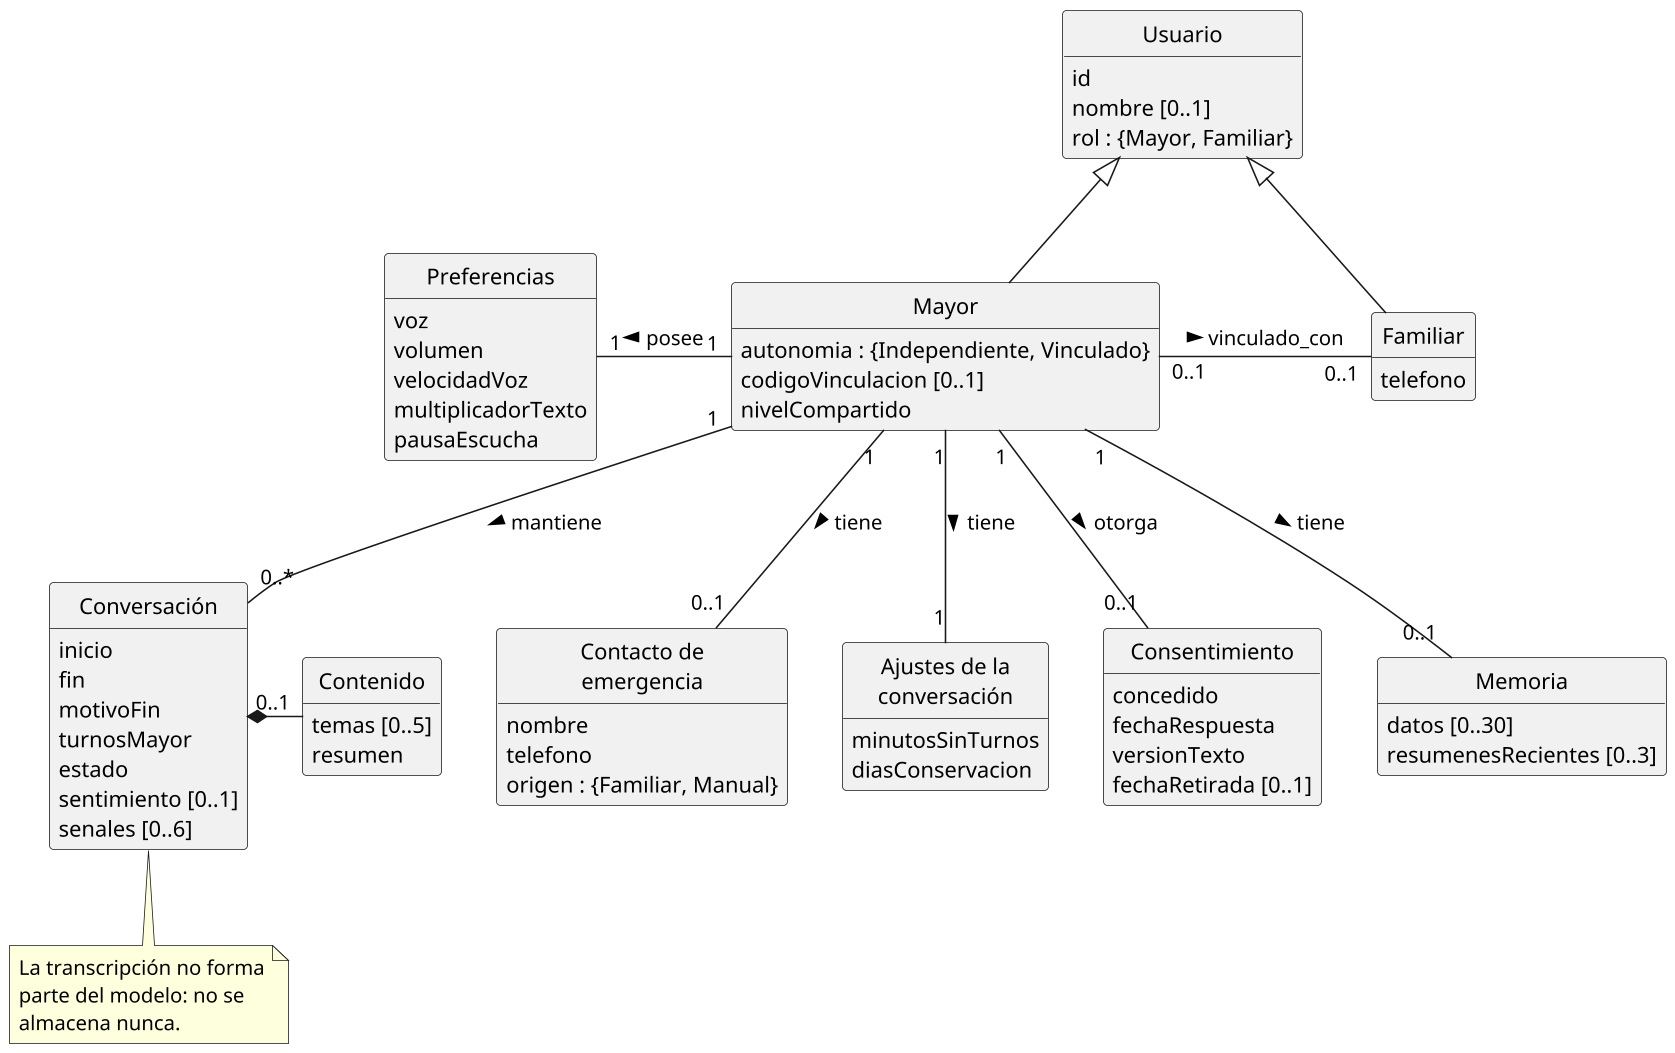
\includegraphics[width=\textwidth]{imagenes/uml/diagrama_conceptual.png}
    \caption{Modelo conceptual de dominio del sistema.}
    \label{fig:dominio}
\end{figure}

El sistema maneja ocho entidades. El \textbf{Usuario} es una persona que usa el sistema, con un rol, \textit{Mayor} o \textit{Familiar}. El mayor tiene además un grado de autonomía, que distingue al independiente del vinculado, y un nivel de compartición, que fija qué parte de su análisis ve el familiar, mientras que el familiar tiene un número de teléfono asociado. Las \textbf{Preferencias} son los ajustes de accesibilidad y de voz del mayor: la voz, su volumen y su velocidad, el multiplicador del tamaño de texto y el tiempo de silencio que cierra su turno. Los \textbf{Ajustes de la conversación} son los dos plazos que gobiernan sus datos: el tiempo sin turnos tras el que una conversación se da por terminada y el tiempo durante el que se conserva lo analizado. El \textbf{Consentimiento} es la respuesta del mayor a la pregunta de si se guardan sus conversaciones, con la fecha en que la dio, la versión del texto que leyó y, si lo retiró, la fecha de retirada. La \textbf{Conversación} es un intercambio entre el mayor y el asistente, delimitado por un periodo sin turnos o por la salida de la aplicación, con sus datos de actividad y el sentimiento y las señales detectados; su \textbf{Contenido}, los temas y el resumen, es una entidad aparte. La \textbf{Memoria} reúne lo que el asistente recuerda del mayor: un conjunto acotado de datos estables y los resúmenes de las últimas conversaciones. El \textbf{Contacto de emergencia}, por último, es la persona a la que el mayor puede llamar desde la pantalla de emergencia, con su nombre, su teléfono y su origen: el familiar, si lo fijó la vinculación, o el propio mayor, si lo introdujo a mano.

La transcripción no forma parte del modelo, pues existe mientras dura la conversación y mientras se analiza, pero no se guarda en ningún soporte. Lo que el sistema almacena es, por tanto, un subconjunto deliberado de lo que maneja, y esa diferencia es la que aplica el principio de minimización de RNF-10. Tampoco es casual que la conversación y su contenido estén separados: corresponden a los dos niveles de lo que el mayor puede compartir con su familiar, y esa separación es la que permite hacerlo cumplir en el servidor (capítulo~\ref{cap:diseno-desarrollo}).

La relación principal es la \textbf{vinculación} entre un mayor y un familiar. Es binaria, bidireccional y opcional, se establece mediante un código temporal de un solo uso y, una vez establecida, autoriza al familiar a leer el perfil del mayor y a modificar sus preferencias, su nombre y los plazos de sus conversaciones, y nada más. Lo que pueda leer del análisis de esas conversaciones depende, además, de lo que el mayor haya decidido compartir.

La cardinalidad $0..1$ en los dos extremos de \textit{vinculado\_con} limita la vinculación a una pareja: cada mayor se vincula como mucho con un familiar, y cada familiar como mucho con un mayor. La restricción simplifica el modelo y las reglas de acceso. Admitir varios familiares por mayor y varios mayores por familiar convertiría la relación en una de muchos a muchos ($0..*$ en los dos extremos), una ampliación que se plantea en el capítulo~\ref{cap:desarrollo-futuro}.
